\documentclass{article}

\usepackage{algorithm2e}
\usepackage{graphicx}
\usepackage{multirow}

\begin{document}

\section{Introduction}
The Full Adder Tree method is a hardware solution for fast multiplication. Suppose you need to multiply two $n$-bit binary numbers. First, a partial product of size $n$~by~$2n-1$ is generated from the numbers. Then, a binary tree of full-adders is constructed with $\lceil~\frac{n}{2}~\rceil$ leaf nodes. Each row of the partial product is fed as an input into one of the leaf full-adders, and each full-adder in the tree performs concurrent addition. The sum bit is propagated to the parent adder, and the carry bit stored internally for the next round of addition. The sum bit of the root node is one column of the final multiplication result. This produces a pipelined architecture where different columns of the partial product are at different heights of the full-adder tree. Table~\ref{FAT_Representation} shows the Full Adder Tree representation for two 4-bit binary numbers, where x corresponds to a bit of the partial product.

\begin{table}[h]
	\begin{center}
	\begin{tabular}{ *{7}{c} | *{2}{c} }
		0&0&0&x&x&x&x & \multirow{2}{*}{FA} & \multirow{4}{*}{FA (solution)} \\
		0&0&x&x&x&x&0 & \\
		0&x&x&x&x&0&0 & \multirow{2}{*}{FA} \\
		x&x&x&x&0&0&0 & \\
	\end{tabular}
	\end{center}
	\caption{Representation of a Full Adder Tree}
	\label{FAT_Representation}
\end{table}

The purpose of this report was to produce a software simulation of Full Adder Tree multiplication and gather experimental results for both the hardware and clock cycle complexity. Hardware complexity refers to the number of full-adders required to perform the multiplication, or the number of full-adder nodes in the binary tree. Hardware complexity does not include the number basic gates required to compute the partial product as the hardware requirements are assumed trivial in comparison to the full-adder. Clock cycle complexity refers to the number of clock cycles required to perform the fast multiplication, in addition to the amount of time required to generate the partial product. Analysis of these two complexities allows for comparison of the Full Adder Tree method with other means of fast multiplication.

A binary tree-based approach was used for the implementation method presented in this report. A node structure was developed where each node maintained an internal full-adder and links to each of its two children. Such an implementation has numerous advantages, which include:

\begin{itemize}
	\item	Accurate simulation of the Full Adder Tree method
	\item Ease of implementation in the C++ language
	\item Natural recursive solution for concurrent addition
\end{itemize}

Both complexities also have natural representations with such a method, as the hardware complexity would be the size of the binary tree and the clock cycle complexity would be proportional to the number of calls made to the root node concurrent addition call. The remainder of this report describes the algorithms used to to implement Full Adder Tree multiplication, the theoretical complexities of the method, and experimental results that verify the theoretical analysis.

\section{Implementation}
This section describes the various algorithms used to implement Full Adder Tree multiplication. The implementation consists of three distinct parts: generation of the partial product used as an input to tree, construction of the binary full-adder tree, and the algorithm to produce the result of multiplication through repeated addition.

\subsection{Partial Product Generation}
The partial product was implemented as a test-and-shift algorithm as presented in Algorithm~\ref{PartialProduct}. An internal variable $entry$ was initialized to the multiplier and a \textbf{for} loop then iterated over each bit of the multiplicand. If the multiplicand bit under consideration was 1, then the $entry$ was copied into the corresponding row of the partial product. Otherwise, the row was left with its default value of all 0's. The $entry$ was shifted to the left before the next multiplicand bit was considered. This implementation represents the natural method of generating a partial product by hand, but does not necessarily resemble the natural hardware solution of bit-wise AND. It was chosen for its simplicity of implementation.

\begin{algorithm}[h]
	\SetKwInOut{Input}{input}
	\SetKwInOut{Output}{output}
	\SetKwData{Entry}{entry}
	\SetKwFunction{Shift}{leftshift}
		
	\Input{A $multiplier$ for the multiplication}
	\Input{A $multiplicand$ for the multiplication}
	\Input{The size $N$ of both of the two inputs}
	\Output{A matrix $M$ of the partial product}
	
	\BlankLine
	\Entry $\leftarrow$ $multiplier$\;
	\BlankLine
	
	\tcp{Pad the entry with zeros}
	\For{$i \leftarrow N+1$ \KwTo $2N-1$}
	{
		\Entry$[i]$ $\leftarrow$ 0\;
	}
	\BlankLine
	
	\For{$i \leftarrow 1$ \KwTo $N$}
	{
		\If{$multiplicand[i] = 1$}
		{
			$M \leftarrow \Entry$\;
		}
		\Shift{\Entry}\;
	}
	\caption{Partial Product Generation}
	\label{PartialProduct}
\end{algorithm}

\subsection{Full Adder Tree Construction}
The binary full-adder tree was generated as a tree structure where each node contained an adder whose input was the output of its two children. In order to account for the leaf-node adders, which had no children, each row of the partial product was represented as a special source node which fed its input into one of the leaf adders. This representation, shown in Figure~\ref{TreeFormat}, used the partial product rows as the actual root nodes of the full-adder tree.

\begin{figure}[h]
	\begin{center}
	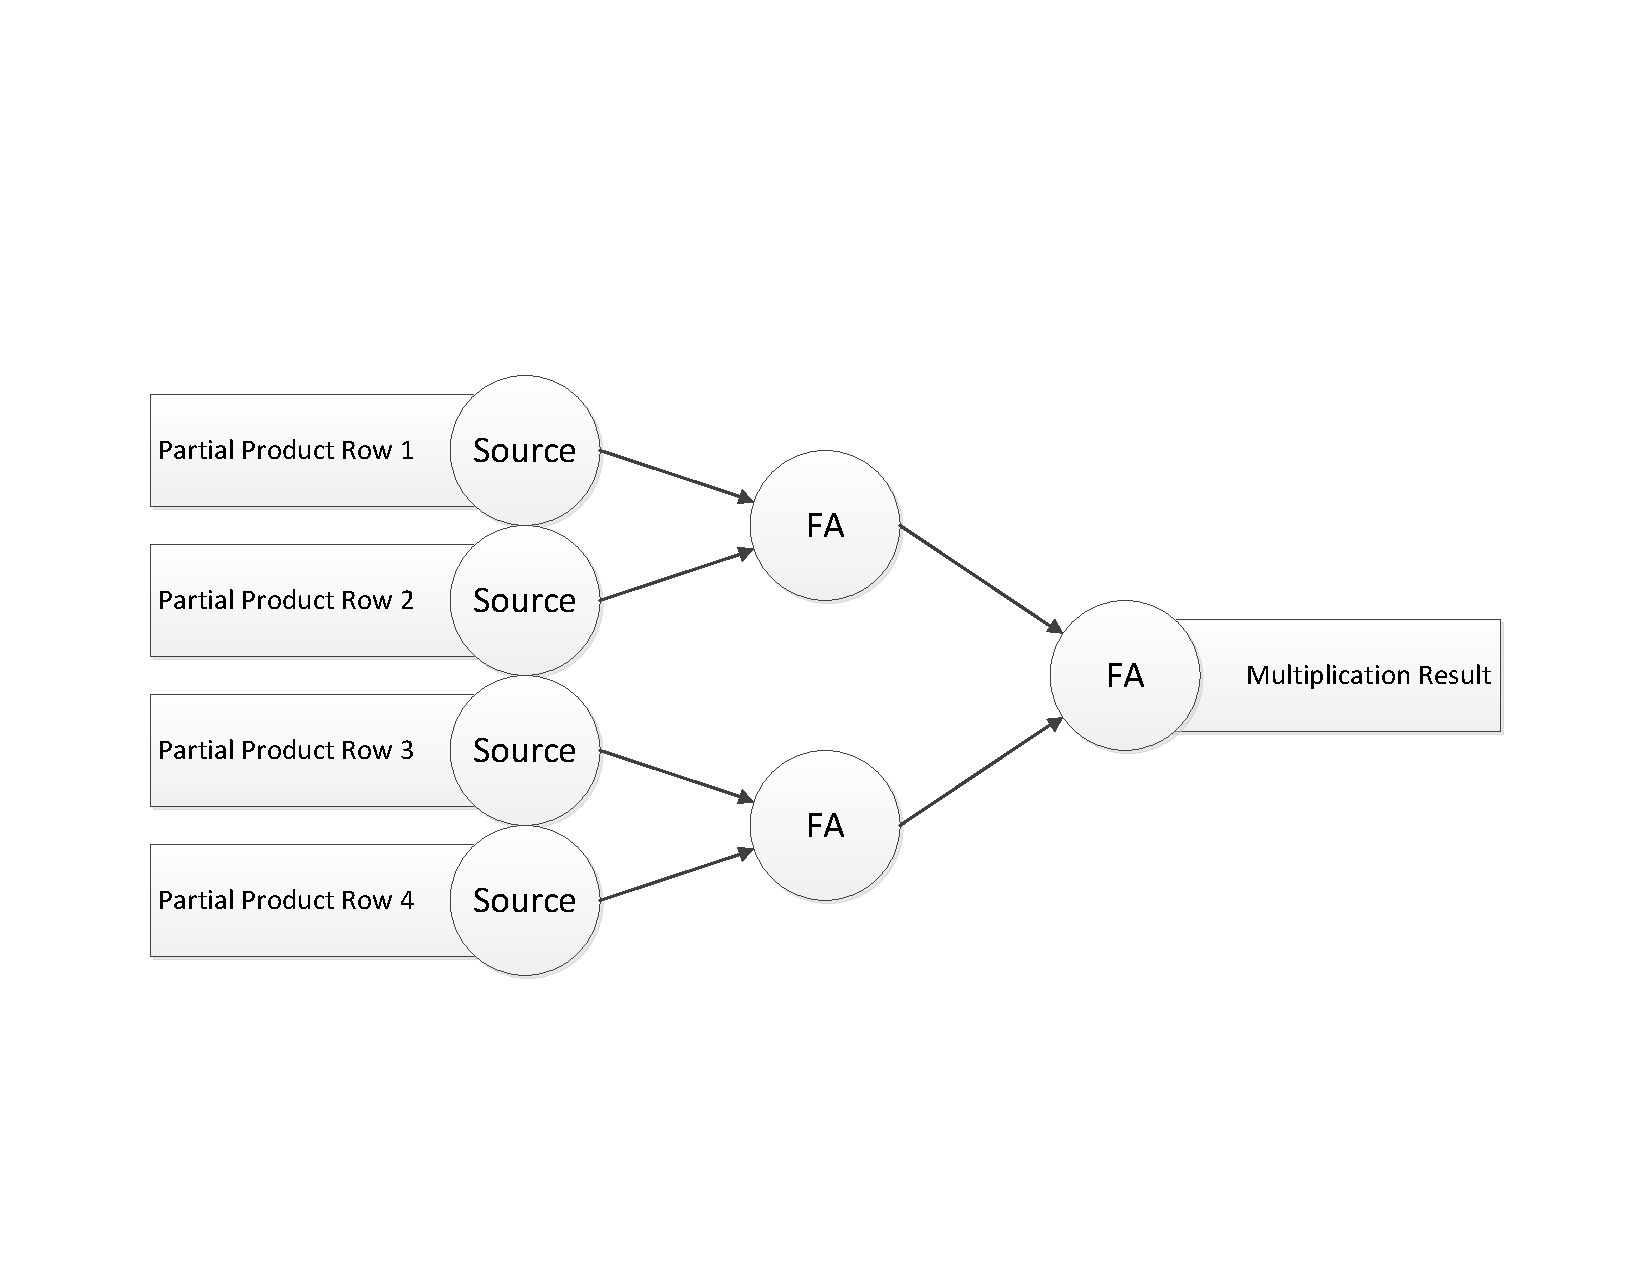
\includegraphics[width=0.8\textwidth]{TreeFormat}
	\end{center}
	\caption{Format of the Full Adder Tree}
	\label{TreeFormat}
\end{figure}

The algorithm to construct the tree in Figure~\ref{TreeFormat} used a bottom-up approach. Each row of the partial product was considered the root of a binary tree with height 1, and each of these trees were added to a queue that represented the forest of trees in consideration. So long as more than one tree existed in the forest, two trees were removed from the queue and used as the children of a new full-adder node. The tree rooted at this new full-adder node was then pushed back onto the queue. The queue size was reduced by 1 each iteration until a single tree, the Full Adder Tree, was in the queue. Algorithm~\ref{TreeConstruction} describes this process.

\begin{algorithm}[h]
	\SetKwInOut{Input}{input}
	\SetKwInOut{Output}{output}
	\SetKwData{Queue}{queue}
	\SetKwData{Adder}{adderNode}
	\SetKwData{Source}{sourceNode}
	\SetKwData{LeftChild}{leftChild}
	\SetKwData{RightChild}{rightChild}
	\SetKwFunction{Front}{front}
	\SetKwFunction{Size}{size}
	\SetKwFunction{Push}{push}
	\SetKwFunction{Pop}{pop}
		
	\Input{A matrix $M$ of the partial product}
	\Input{The size $N$ of the multiplier}
	\Output{The $root$ of a full-adder tree}
	
	\BlankLine
	\For{$i \leftarrow 1$ \KwTo $N$}
	{
		\tcp{Create source from row of partial product}
		\Source $\leftarrow M[i]$\;
		\Push{\Queue,\Source}\;
	}
	\BlankLine
	
	\While{\Size{\Queue} $>$ 1}
	{
		\tcp{Get left input to new full adder}
		\LeftChild $\leftarrow$ \Front{\Queue}\;
		\Pop{\Queue}\;
		\BlankLine
		\tcp{Get right input to new full adder}
		\RightChild $\leftarrow$ \Front{\Queue}\;
		\Pop{\Queue}\;
		\BlankLine
		\tcp{Create full adder from two input sources}
		\Adder $\leftarrow$ (\LeftChild,\RightChild)\;
		\Push{\Queue,\Adder}\;
	}
	\BlankLine
	
	$root \leftarrow$ \Front{\Queue}\;
	\caption{Full Adder Tree Construction}
	\label{TreeConstruction}
\end{algorithm}

\subsection{Recursive Multiplication}
The multiplication algorithm was implemented as a series of concurrent additions, where each addition was a recursive call that began at the root node and propagated down the tree breadth-first. After each addition, the full-adder nodes sent a signal to their parents that indicated whether a new output was produced. This signal determined which adders would participate in the next round of addition. Termination was detected when no signal was produced by any adder in the tree, indicating that no more bits were being propagated towards the root.

When the root node produced a result, it was extracted from the tree and stored in the result register. When termination was detected, the carry bit of the root adder was extracted and used as the last bit of the result. This final operation was not considered for the clock cycle complexity of the algorithm since it could be gated into the next bit of the result register without the need for an additional clock cycle. This assumption is expressed in the section on complexities.

Algorithm~\ref{RecursiveRoot} describes the root-level call of the multiplication function. Algorithm~\ref{RecursiveNode} describes the recursive implementation at each full-adder node. Note that the algorithm for the source partial product nodes is not described, as its sole operation was to produce and consume an output when prompted. Also note that the pseudocode for these algorithms has been simplified for the purposes of presentation. In particular, the internal storage of the result has been omitted as well as the requirement that an adder node not produce a new result until its old result has been consumed. These features are crucial for the correct performance of the algorithm, but not for understanding of its implementation.

\begin{algorithm}[h]
	\SetKwInOut{Input}{input}
	\SetKwInOut{Output}{output}
	\SetKwData{Index}{index}
	\SetKwFunction{GetCarry}{GetCarry}
	\SetKwFunction{HasResult}{HasResult}
	\SetKwFunction{GetResult}{GetResult}
	\SetKwFunction{Add}{RecursiveAdd}
		
	\Input{A $root$ of the full adder tree}
	\Output{A $result$ of the multiplication}
	
	\BlankLine
	\Index $\leftarrow 1$\;
	\While{\Add{$root$} does not terminate}
	{
		\If{\HasResult{$root$}}
		{
			$result[\Index] \leftarrow$ \GetResult{$root$}\;
			\Index $\leftarrow \Index+1$\;
		}
	}
	$result[\Index] \leftarrow$ \GetCarry{$root$}\;
	\caption{Root-Level Multiplication}
	\label{RecursiveRoot}
\end{algorithm}

\begin{algorithm}[h]
	\SetKw{And}{and}
	\SetKwInOut{Input}{input}
	\SetKwData{Left}{LeftChild}
	\SetKwData{Right}{RightChild}
	\SetKwFunction{Result}{HasResult}
	\SetKwFunction{Add}{PerformAddition}
	\SetKwFunction{Notify}{NotifyParent}
	\SetKwFunction{RecAdd}{RecursiveAdd}
	
	\Input{An operand $lhs$ from the left child}
	\Input{An operand $rhs$ from the right child}
	
	\BlankLine	\If{\Result{\Left} \And \Result{\Right}}
	{
		\Add{$lhs$,$rhs$}\;
		\Notify{}\;
	}
	\RecAdd{\Left}\;
	\RecAdd{\Right}\;
	\caption{RecursiveAdd Pseudocode}
	\label{RecursiveNode}
\end{algorithm}

\section{Theoretical Analysis}
In order to verify the correctness of the implementation described above, a number of theoretical equations were derived to determine the actual hardware and clock cycle complexity expected from a Full Adder Tree implementation. Numerical correctness was verified using a set of sample data with known outputs, and is not described by this report, although it can be verified using the numerical data provided in the experimental results.

\subsection{Hardware Complexity}
The hardware complexity can be demonstrated through a simple inductive proof. Assume that the hardware complexity of a full adder tree for an $n$-bit multiplicand is $n-1$.

\textbf{Base Case:} Let $n = 2$. The partial product consists of a matrix with 2 rows and 3 columns. In order to generate the result, each row of the partial product must be fed into a full adder. A single full adder can be used to generate this result, since a full adder has two input pins and there are two rows that need to be added. Therefore, 1 full adder is sufficient for the base case. The base case holds as the hardware complexity is $n-1$.

\textbf{Inductive Step:} Suppose the inductive hypothesis is true for $n-1$. The partial product for the case $n$ has one additional row over the case $n-1$, since one additional bit of the multiplicand must be considered. Using the full adder tree from the case for $n-1$, which contained $n-2$ full adders based on the supposition, all rows of the partial product except for this newly added row are connected in a binary full-adder tree. Add 1 full-adder that connects the root of this full-adder tree with the additional row in the partial product. This new full-adder tree connects all rows of the partial product to the result, and does so with 1 additional adder over the $n-1$ case. Since the $n-1$ case contained $n-2$ adders, the $n$ case contains $n-1$ adders. The inductive step holds.

This proof shows that the hardware complexity of a Full Adder Tree for an input of size $n$ is $n-1$, assuming the two inputs are uniform and only the full adders contribute to the complexity. This equation was used to verify the hardware complexity produced by the experimental results.

\subsection{Clock Cycle Complexity}
The clock cycle complexity of the algorithm becomes simple once the algorithm is phrased as a pipelined execution. Observe that the binary full-adder tree in Figure~\ref{TreeFormat} consists of a tree of some height $h$ where $h = 3$. A critical path, or the longest path, from the partial product to the multiplication result is the height $h$. However, note that the source nodes do not perform addition and therefore do not contribute to the complexity of the implementation, resulting in $h-1$ levels of full-adder addition. The propagation delay for the first bit of the partial product to reach the root full adder from the critical path is $h-2$, since the root level can be subtracted from the $h-1$ levels of full-adder addition. This means it takes $h-2$ levels of multiplication for the first bit of the multiplication result to be produced.

Further note that there are $m$ bits of partial product to sum, and the bits are pipelined to arrive one addition after the next. It therefore takes the root full adder $h-2+m$ additions to produce the final result, $h-2$ due to the propagation delay and $m$ to perform the addition. As seen in Table~\ref{FAT_Representation}, the number of bits in each row of the partial product is $2n-1$ where $n$ is the size of the multiplier and the multiplicand. This produces a total number of $2n+h-3$ additions, where $h$ once again represents the height of the full adder tree including an additional level of fake source nodes that add zero complexity. If we ignore the implementation details imposed by this report, the equation would generalize to $2n+h-2$.

Each full adder addition takes $4\Delta t$ and the partial product generation takes $\Delta t$. There are a total of $2n+h-2$ additions. The height of a binary tree is $lgn$. Combined, this produces a clock cycle complexity of $(2n+lgn-2)*4\Delta t + \Delta t$. This equation was used to verify the results produced in the experimental section.

\end{document}